%\documentclass[mathserif]{beamer}
\documentclass[handout]{beamer}
%\usetheme{Goettingen}
%\usetheme{Warsaw}
\usetheme{Singapore}



%\usetheme{Frankfurt}
%\usetheme{Copenhagen}
%\usetheme{Szeged}
%\usetheme{Montpellier}
%\usetheme{CambridgeUS}
%\usecolortheme{}
%\setbeamercovered{transparent}
\usepackage[english, activeacute]{babel}
\usepackage[utf8]{inputenc}
\usepackage{amsmath, amssymb}
\usepackage{dsfont}
\usepackage{graphics}
\usepackage{cases}
\usepackage{graphicx}
\usepackage{pgf}
\usepackage{epsfig}
\usepackage{amssymb}
\usepackage{multirow}	
\usepackage{amstext}
\usepackage{algorithm2e}
\usepackage{amsmath}
\usepackage{epic}
\usepackage{epsfig}
\usepackage{fontenc}
\usepackage{framed,color}
\usepackage{palatino, url, multicol}
%\algsetup{indent=2em}
\newcommand{\factorial}{\ensuremath{\mbox{\sc Factorial}}}
\newcommand{\BIGOP}[1]{\mathop{\mathchoice%
{\raise-0.22em\hbox{\huge $#1$}}%
{\raise-0.05em\hbox{\Large $#1$}}{\hbox{\large $#1$}}{#1}}}
\newcommand{\bigtimes}{\BIGOP{\times}}
\vspace{-0.5cm}
\title{Academic Position Job Interview\\ DCC - University of Chile}
\vspace{-0.5cm}
\author[Felipe Bravo Márquez]{Felipe Bravo Márquez}
 


\date{2 October, 2018}

\begin{document}
\begin{frame}
\titlepage


\end{frame}


%presente su CV, sus líneas de investigación y su plan académico (investigación y docencia).


\section{CV}


\begin{frame}{About me}
\begin{scriptsize}
\begin{itemize}
 \item I'm a research fellow in the Machine Learning Group at the University of Waikato. 
 \item I conducted my PhD in the same lab under the supervision of Bernhard Pfahringer and Eibe Frank.
 \item This is a very prestigious research group in Machine Learning where two internationally successful open source machine learning software suites WEKA and MOA were developed. 
 \item My research interests and expertise lie in the acquisition of knowledge and information from unstructured data, particularly natural language text, spanning the following overlapping fields:
\begin{enumerate}
\begin{scriptsize}
 \item  Natural language processing
 \item  Machine learning
 \item Artificial Intelligence
 \end{scriptsize}
\end{enumerate}

\item My main research goals are to study society by computationally analyzing language traces left by humans in the digital space.


\end{itemize}


\end{scriptsize}

\end{frame}






\begin{frame}{Qualifications}
\begin{scriptsize}
  \begin{enumerate}
\item[2014-2017] PhD in Computer Science, The University of Waikato, New Zealand.

\item[2011-2013] M.Sc. in Computer Science, University of Chile (summa cum laude).

\item[2010] Professional Degree in Industrial Engineering, University of Chile (summa cum laude).

\item[2010] Professional Degree in Computer Science Engineering, University of Chile (summa cum laude).

\item[2005-2009]  Bachelor of Science in Industrial Engineering, University of Chile.

\item[2003-2008]  Bachelor in Computer Science, University of Chile.
  \end{enumerate} 
\end{scriptsize}

\end{frame}




\begin{frame}{Work Experience}
\begin{scriptsize}
  \begin{enumerate}
\item[ 2017-] Research Fellow, \textit{Machine Learning Group, University of Waikato}. \\
\item[2011-2013] Research Engineer, \textit{Yahoo! Labs Latin America}. \\ \url{http://labs.yahoo.com/Yahoo_Labs_Santiago} 
\item[2009- 2011] Researcher and Software Developer, \textit{Web Intelligence Consortium Chile Research Centre}.    \\ \url{http://wi.dii.uchile.cl}
\item[2009] Internship, \textit{Simple}, Software Developer. \\ \url{http://www.simple.cl}.
\item[2009] Internship, \textit{Previred}, Business Process Management Area. \\ \url{http://www.previred.com}.
\item[2005-2006] Internship, \textit{Vitanet}, Software Developer. \\ \url{http://www.vitanet.cl}. 
  \end{enumerate} 
\end{scriptsize}

\end{frame}

\begin{frame}{Scholarships, Grants, etc}
\begin{scriptsize}
  \begin{enumerate}
 \item[2018] Nominated by the University of Waikato for the Doctoral Dissertation Award at iConference 2019.
 \item[2018] Passed to second round on a Marsden Grant funded by the Royal Society of New Zealand.
\item[2017] University of Waikato Doctoral Publications Scholarship.

\item[2016] IEEE student travel grant to attend the 2016
IEEE/WIC/ACM International Conference on Web Intelligence in Omaha, Nebraska, USA.

\item[2014-2017]  University of Waikato Doctoral Scholarship.

\item[2011-2012]  National Scientific and Technological Research Commission (CONICYT) Scholarship for master's degree studies at Chilean Universities.
  \end{enumerate} 
\end{scriptsize}

\end{frame}





\begin{frame}{Selected Publications}
\begin{scriptsize}
\begin{enumerate}
\item F. Bravo-Marquez, E. Frank, and B. Pfahringer \textit{Building a Twitter Opinion Lexicon from Automatically-annotated Tweets}, In \textit{Knowledge-Based Systems}  Volume 108, September 2016, Pages 65–78.
\item F. Bravo-Marquez, M. Mendoza and B. Poblete \textit{Meta-Level Sentiment Models for Big Social Data Analysis}, In \textit{Knowledge-Based Systems} Volume 69, October 2014, Pages 86–99. 
\item S. M. Mohammad, F. Bravo-Marquez, M. Salameh, and S. Kiritchenko  \textit{Semeval-2018 Task 1: Affect in tweets}. In \textit{Proceedings of International Workshop on Semantic Evaluation (SemEval-2018)}, New Orleans, LA, USA, June 2018. 
\item F. Bravo-Marquez, E. Frank, and B. Pfahringer \textit{Positive, Negative, or Neutral: Learning an Expanded Opinion Lexicon from Emoticon-annotated Tweets}, In \textit{IJCAI '15: Proceedings of the 24th International Joint Conference on Artificial Intelligence}. Buenos Aires, Argentina 2015.
\item F. Bravo-Marquez, E. Frank, and B. Pfahringer \textit{Annotate-Sample-Average (ASA): A New Distant Supervision Approach for Twitter Sentiment Analysis}, In \textit{The biennial European Conference  on Artificial Intelligence (ECAI'16)}. The Hague, Netherlands.
\item F. Bravo-Marquez, E. Frank, and B. Pfahringer \textit{From Unlabelled Tweets to Twitter-specific Opinion Words}, In \textit{SIGIR '15: Proceedings of the 38th International ACM SIGIR Conference on Research \& Development in Information Retrieval}. Santiago, Chile 2015.  
\end{enumerate} 
\end{scriptsize}
\end{frame}




\begin{frame}{Citations}
\begin{figure}[htb]
	\centering
	 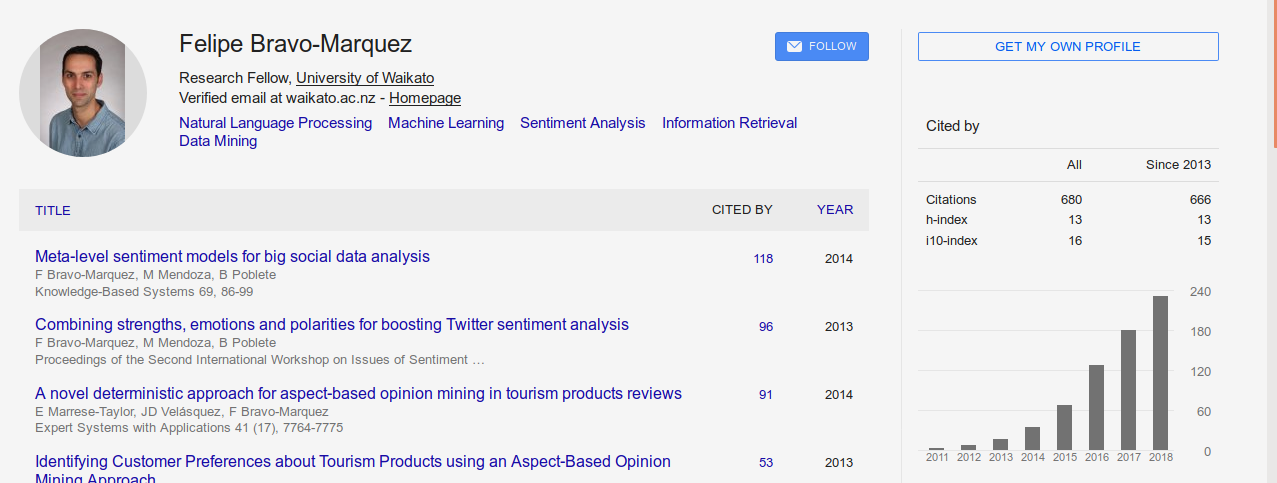
\includegraphics[scale=0.35]{pics/gscholar.png}
\end{figure}
\end{frame}



\begin{frame}{Teaching}
\begin{scriptsize}
  \begin{enumerate}
\item [Spring 2018] (Lecturer) Practical Data Mining (COMP321), The University of Waikato

\item [June 2018] (Lecturer) Deep Learning for Natural Language Processing, IfI Summer School 2018 on Machine Learning,  Deparment of Informatics, University of Zurich. 

\item[Spring 2013] (Lecturer) Databases Management Diploma, Informatics Engineering Department (postgraduate), Universidad Técnica Federico Santa María.

\item[Spring 2012] (Lecturer) Data Mining (CC5206/CC71Q), Computer Science Department (undergraduate and postgraduate), University of Chile.

\item[Fall 2011]   (Lecturer) Information Technologies and Business Process Redesign (IN72K), Master in Operations Management, University of Chile.
  \end{enumerate} 
\end{scriptsize}

\end{frame}




\begin{frame}{Student Supervision}
\begin{scriptsize}
  \begin{enumerate}
\item (2018) Nicole Chan, Co-supervised with Andreea Calude, ``Social Media Meets Te Reo  M\={a}ori Loanwords''  Honours Project, University of Waikato. 
\item  (2018)  Joshua Lovelock, Co-supervised with Eibe Frank,``Automatic Detection of Hate Speech'', Honours Project, University of Waikato.
\item  (2018) Tristan Anderson, Co-supervised with Bernhard Pfahringer, ``Building Time-Evolving Opinion Lexicon'', Honours Project, University of Waikato.
\item (2013) Edison Marrese Taylor, Co-supervisor with Juan Velásquez, ``Diseño e Implementación de una Aplicación de Web Opinion Mining para Identificar Preferencias de Usuarios sobre Productos Turísticos de la X Región de los Lagos'', Industrial Engineering, U. of Chile.
\item (2012) Luis Maldonado, Co-supervisor with Mauricio Marín, ``Análisis de Sentimiento en el Sistema de Red Social Twitter'', Execution Informatic Engineering, U. of Santiago.
  \end{enumerate} 
\end{scriptsize}

\end{frame}




\begin{frame}{Professional Community Involvement}
\begin{scriptsize}
  \begin{enumerate}
  \item Co-organizer of the SemEval-2018 Task 1: Affect in Tweets (about 200 participants).
  \item Co-organizer of the WASSA-2017 shared task on emotion intensity (EmoInt).
  \item Program committees: WASSA 2018, WISDOM 2018, SEM-EVAL 2018, IJCAI-ECAI 2018, EMNLP 2017, WASSA 2017.
  \item Journal Reviewer:  Journal of Machine Learning Research, Natural Language Engineering, IEEE Transactions on Knowledge and Data Engineering, Knowledge-based Systems, ACM Transactions on Intelligent Systems and Technology (TIST), IEEE Computational Intelligence Magazine.
  \end{enumerate} 
\end{scriptsize}

\end{frame}





\begin{frame}{Academic Visits}
\begin{scriptsize}
  \begin{enumerate}
\item July 2018 - Institute of Computational Linguistics, University of Zurich, hosted by Martin Volk.
\item September 2017 - Institute of Computational Linguistics, University of Zurich, hosted by Manfred Klenner.
\item October 2016 - National Research Council Canada (NRC), hosted by Saif Mohammad.
  \end{enumerate} 
\end{scriptsize}

\end{frame}





\begin{frame}{Invited Talks}
\begin{tiny}
  \begin{enumerate}
\item [March 2018] Natural Language Processing in NZ Meetup. Tutorial: Using Sentiment Analysis as a Case Study for Introducing Modern NLP Concepts.

\item [February 2018] University of Waikato. Tutorial: Using Sentiment Analysis as a Case Study for Introducing Modern NLP Concepts.

\item [January 2018]Universidad de Chile. Tutorial: Using Sentiment Analysis as a Case Study for Introducing Modern NLP Concepts.

\item [January 2018] Pontifica Universidad Catolica de Chile. Invited talk at CIWS Workshop - Future of Data: Emotion Intensties of Tweets.

\item [September 2017] Institute of Computational Linguistics, University of Zurich:  Acquiring and Exploiting Lexical Knowledge for Twitter Sentiment Analysis.

\item [October 2016] National Research Council Canada (NRC):  Acquiring and Exploiting Lexical Knowledge for Twitter Sentiment Analysis.

\item [September 2016] University of Melbourne, hosted by Timothy Baldwin: Acquiring and Exploiting Lexical Knowledge for Twitter Sentiment Analysis.

\item [July 2016] Pontifica Universidad Catolica de Chile:  Acquiring and Exploiting Lexical Knowledge for Twitter Sentiment Analysis.

\item [July 2016] Universidad de Chile:  Acquiring and Exploiting Lexical Knowledge for Twitter Sentiment Analysis.

\item [June 2016] Universidad Técnica Federico Santa María: Acquiring and Exploiting Lexical Knowledge for Twitter Sentiment Analysis. 
  \end{enumerate} 
\end{tiny}

\end{frame}



\section{My Research}






\begin{frame}{Problem: Affect Classification}
\begin{scriptsize}
  \begin{enumerate}
   \item Automatically map natural language text (e.g., a tweet, a word) into affective states (e.g., anger, fear, positive, negative).
   
     \begin{figure}[h]
        	
\includegraphics[scale = 0.15]{pics/sent.png}
        \end{figure}
   \item State-of-the-art solutions use \textbf{supervised} machine learning models trained from \textbf{manually} annotated examples.
   \item \textbf{Label sparsity problem (LS)}: manual annotation is \textbf{labor-intensive} and \textbf{time-consuming}. 
  \end{enumerate} 
\end{scriptsize}

\end{frame}



\begin{frame}{PhD Dissertation}

My thesis addressed the label sparsity problem for Twitter sentiment classification by automatically building \textbf{two type of resources}. 
\begin{enumerate}
 \item \textbf{Twitter-specific opinion lexicons}: we develop machine learning models to induce polarity lexicons from tweets. 
 \item  \textbf{Synthetically labeled tweets}: we develop distant supervision methods based on \textbf{lexical knowledge} (we go beyond emoticons). 
 \end{enumerate}

\end{frame}




\begin{frame}{Word-sentiment Associations for Polarity Lexicon Induction}
\begin{figure}[htb]
	\centering
	 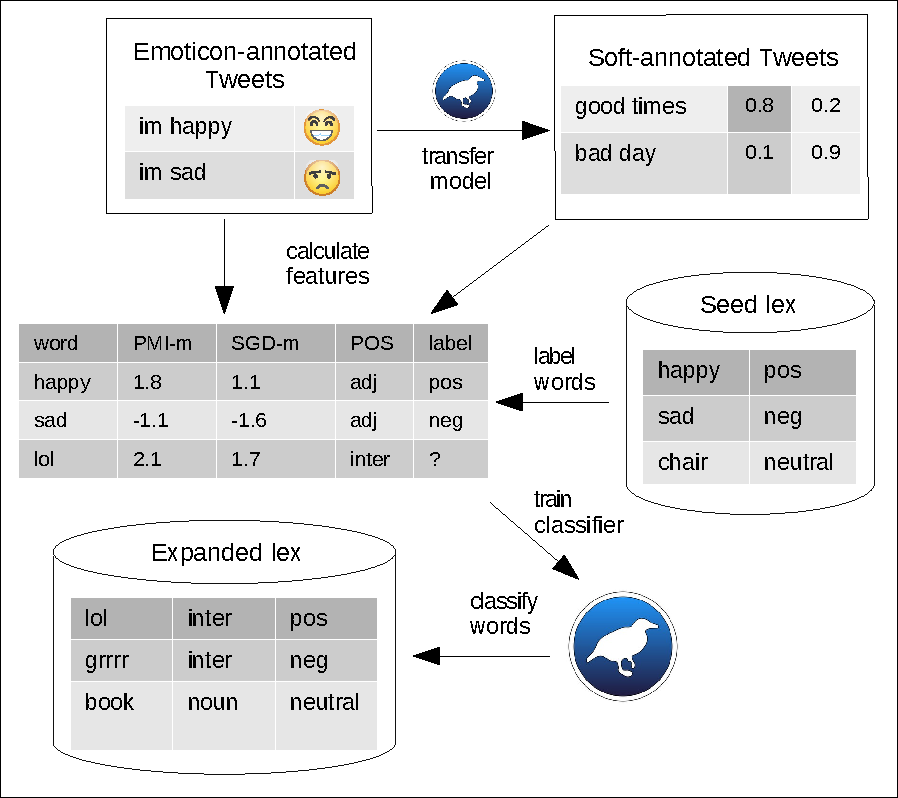
\includegraphics[scale=0.5]{pics/diagramcrop.pdf}
	\label{fig:sosgd}
\end{figure}
\end{frame}







\begin{frame}{Tweet-centroid Model for Lexicon Induction}

\begin{figure}[htb]
	\centering
	 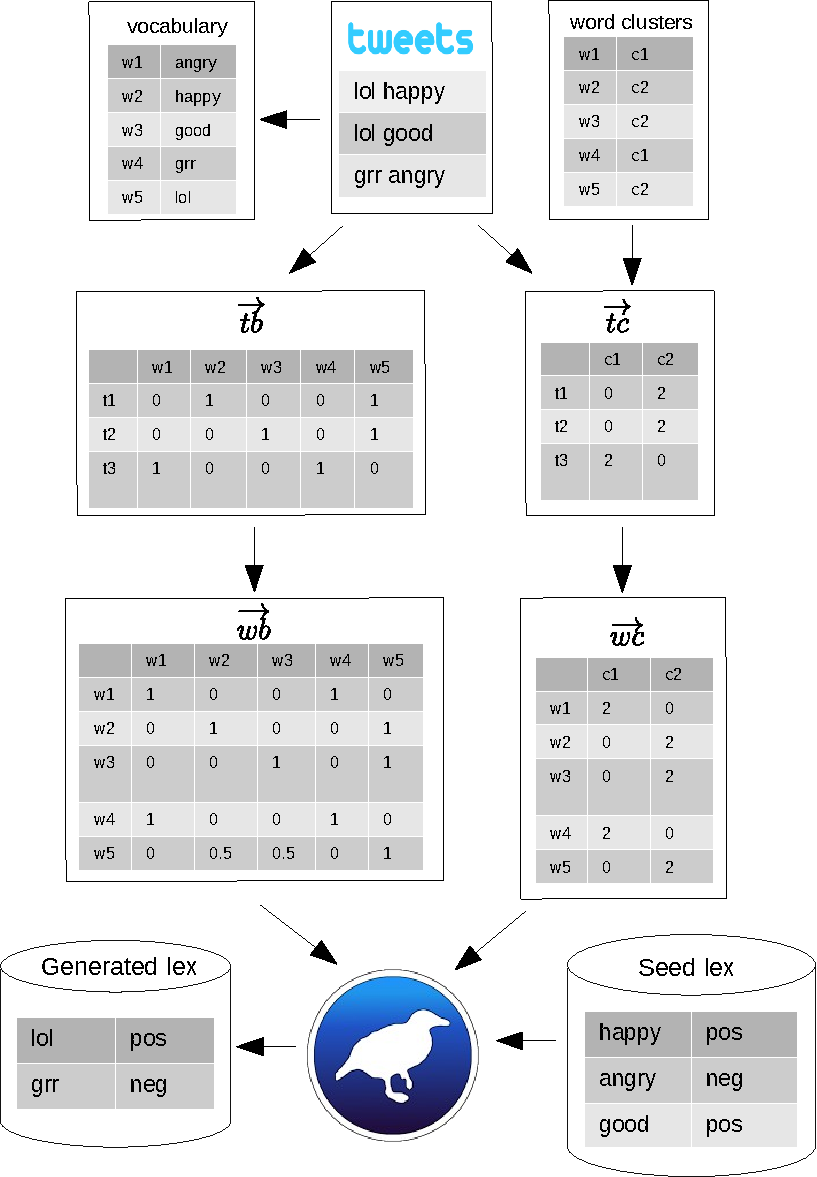
\includegraphics[scale=0.4]{pics/sigirmodel.pdf}
\end{figure}



\end{frame}


\begin{frame}{Multi-Label Classification of Emotions with TCM}
\begin{scriptsize}

\begin{figure}[htbp]
\begin{center}
\scalebox{0.7}{
\begin{tabular}{cccc}
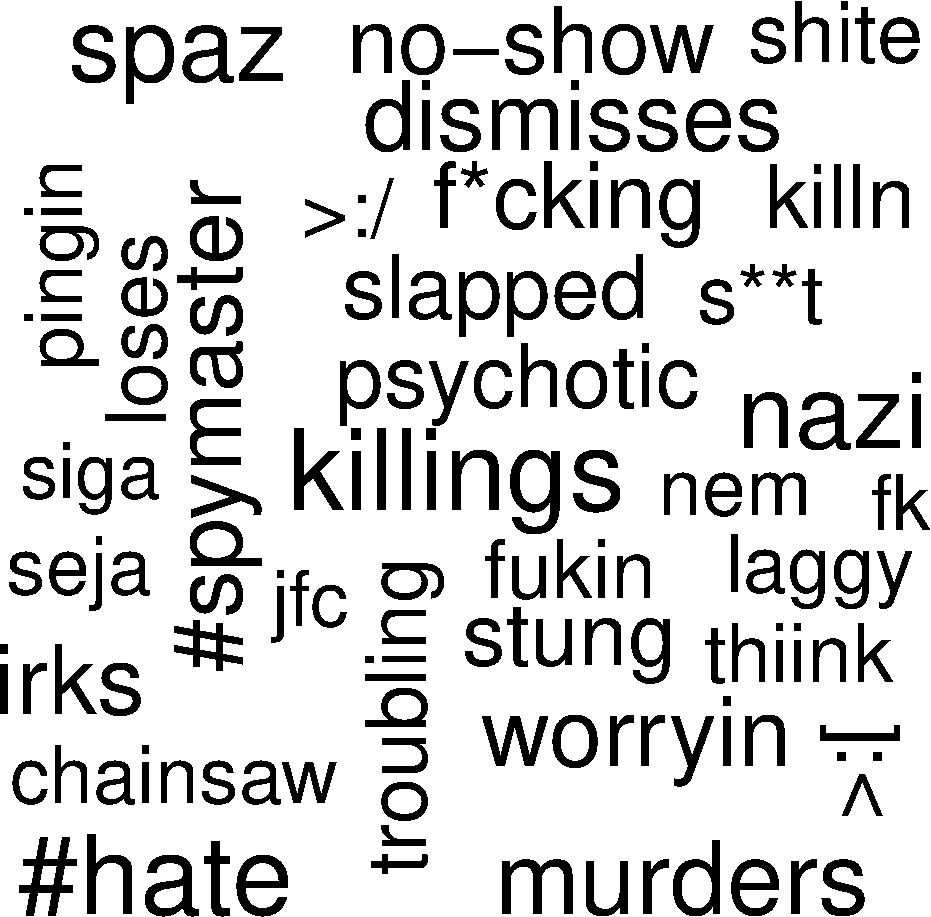
\includegraphics[scale=0.2]{pics/anger.pdf} & 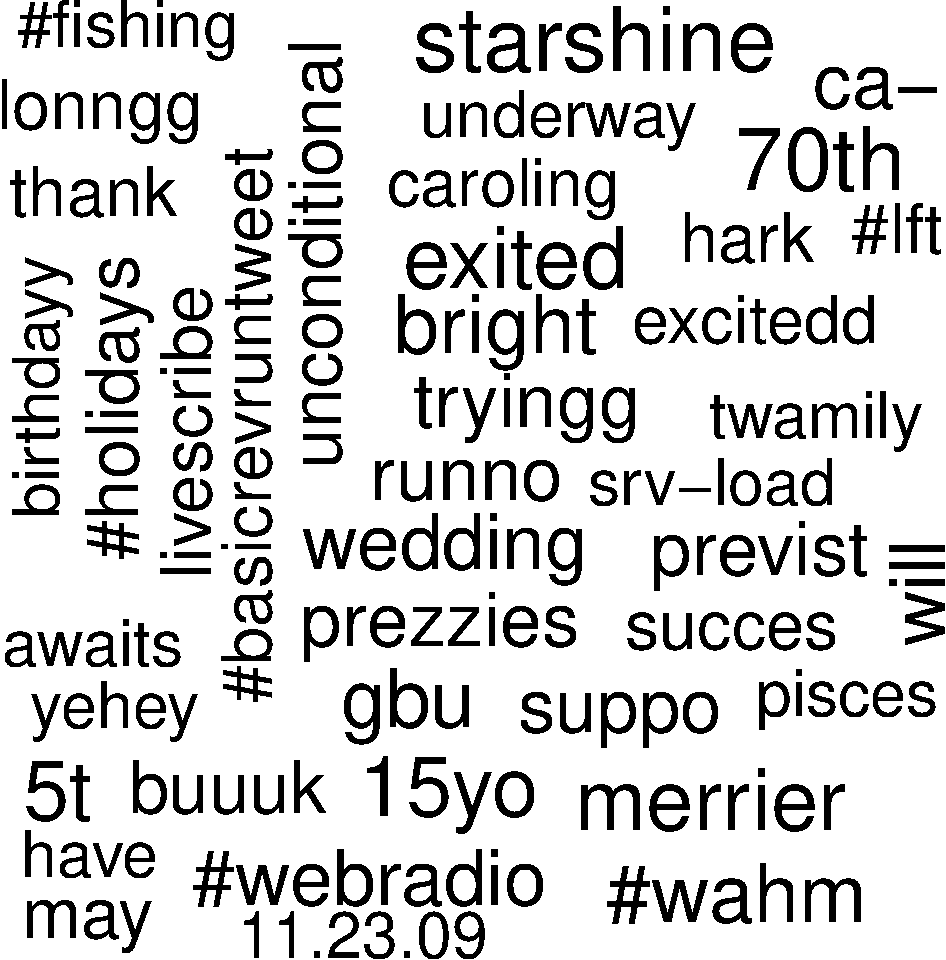
\includegraphics[scale=0.2]{pics/ant.pdf} & 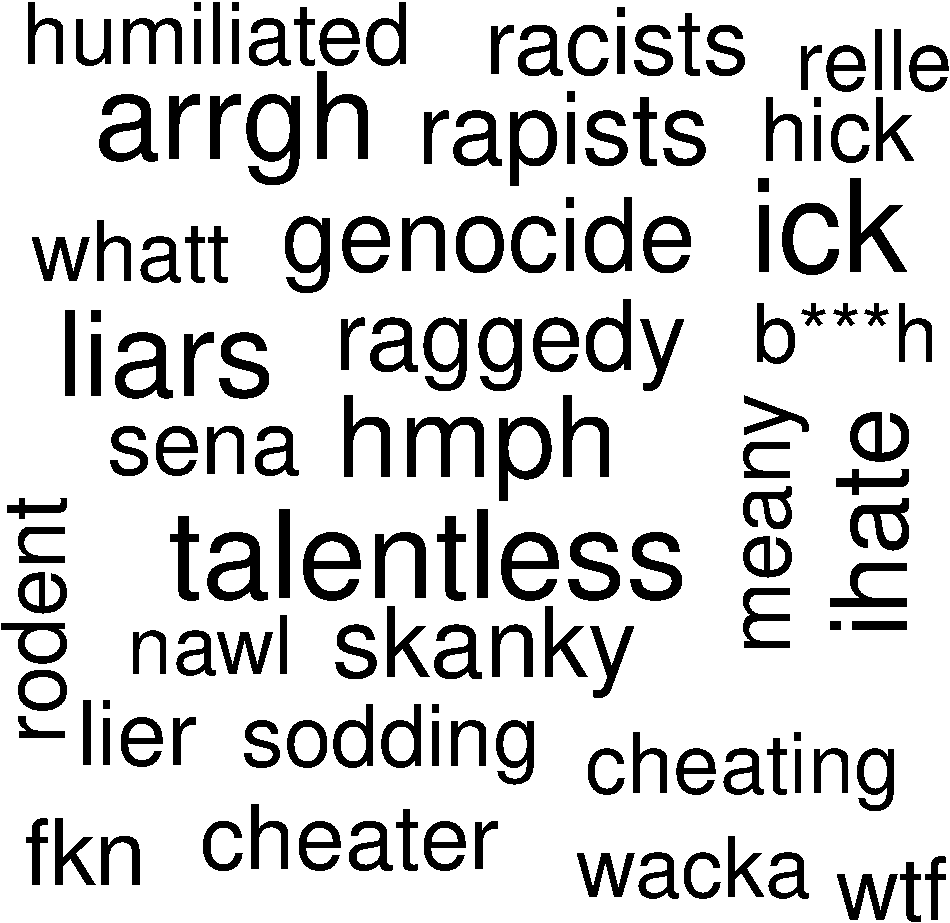
\includegraphics[scale=0.2]{pics/disg.pdf} & 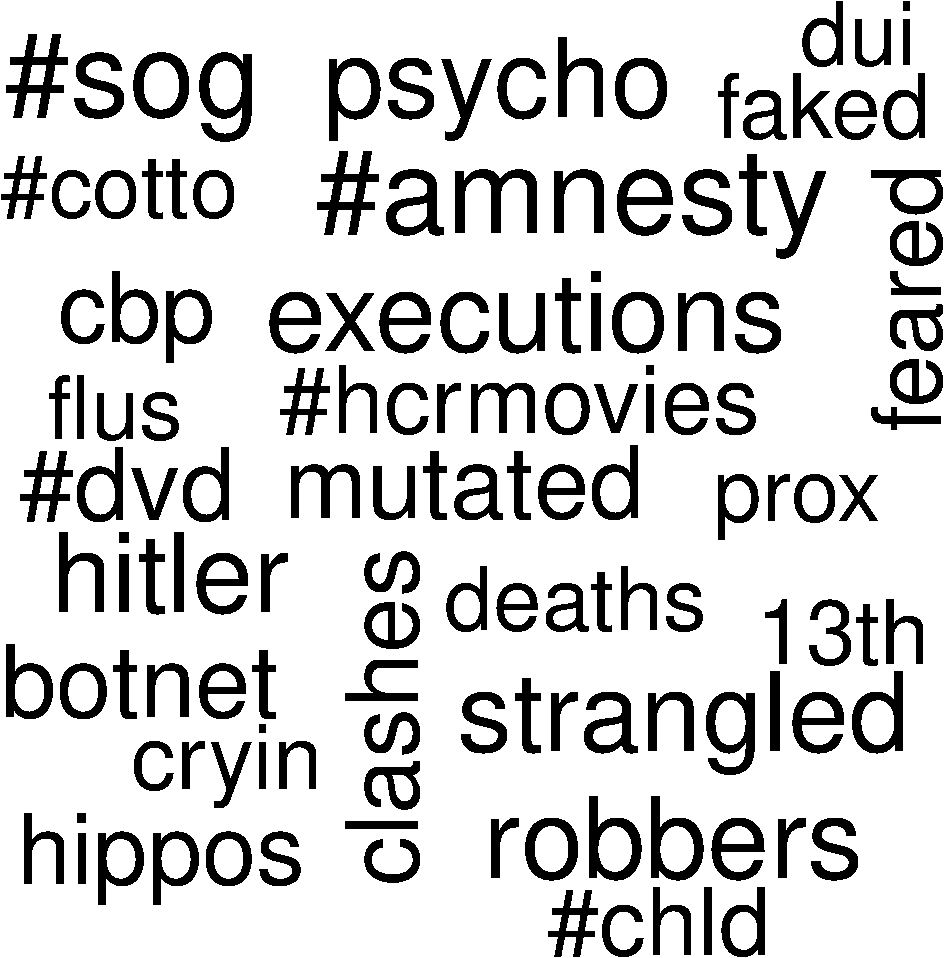
\includegraphics[scale=0.2]{pics/fear.pdf} \\
anger & anticipation & disgust & fear\\[1mm] 
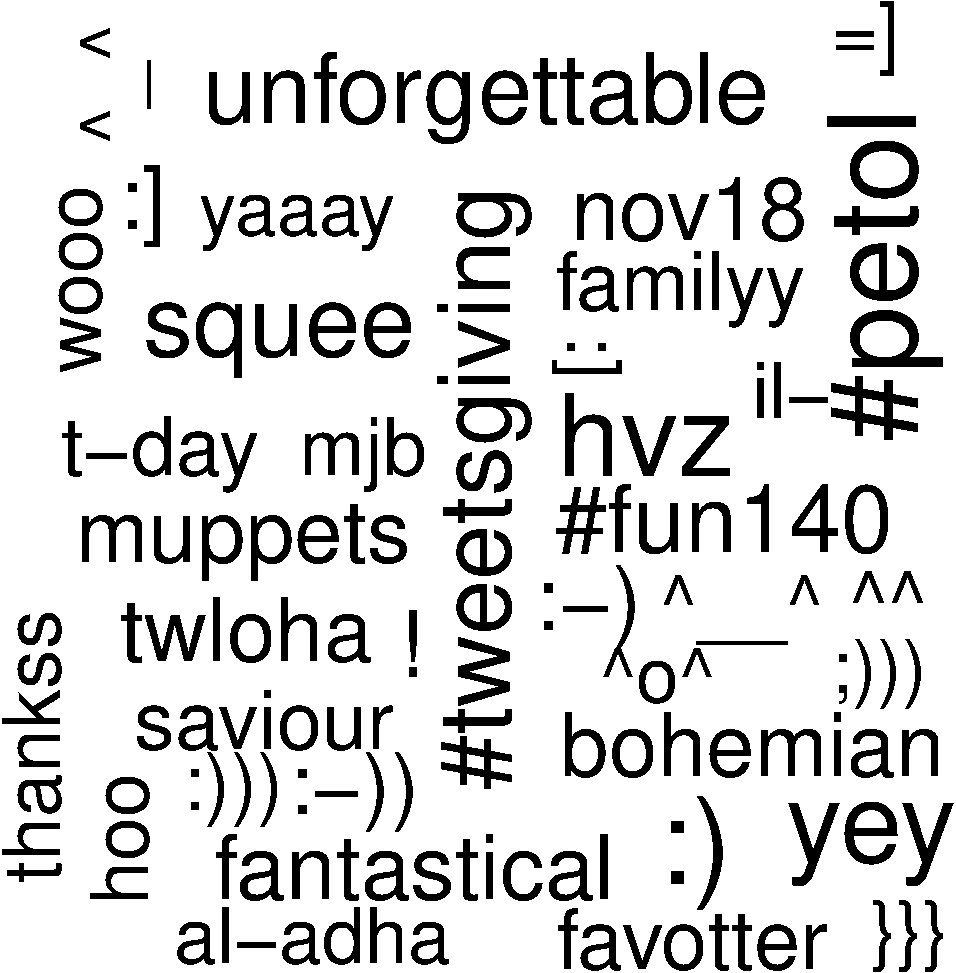
\includegraphics[scale=0.2]{pics/joy.pdf} & 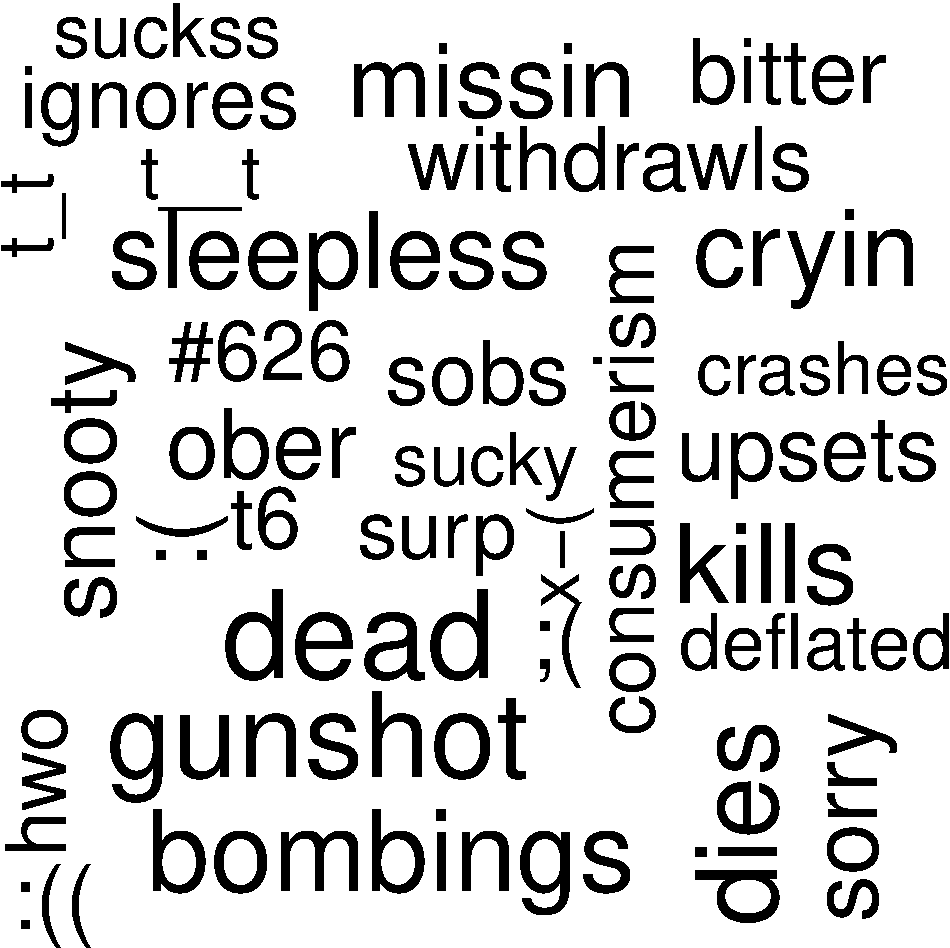
\includegraphics[scale=0.2]{pics/sadness.pdf} & 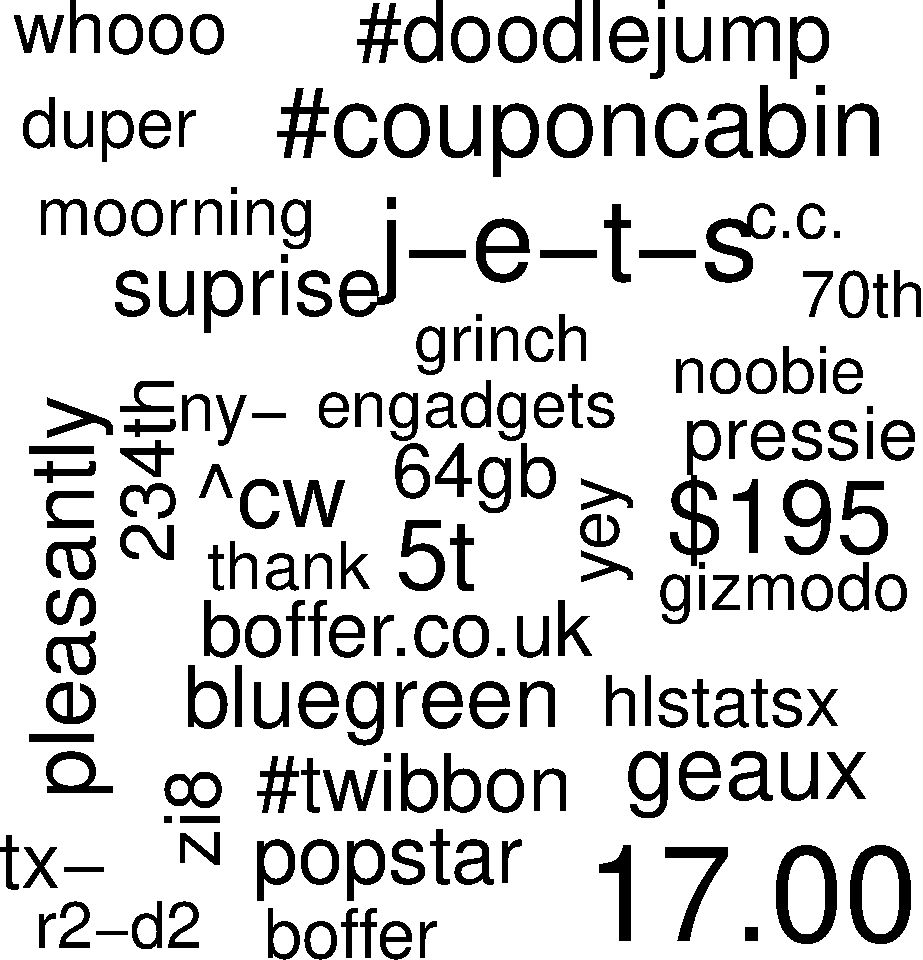
\includegraphics[scale=0.2]{pics/surprise.pdf} & 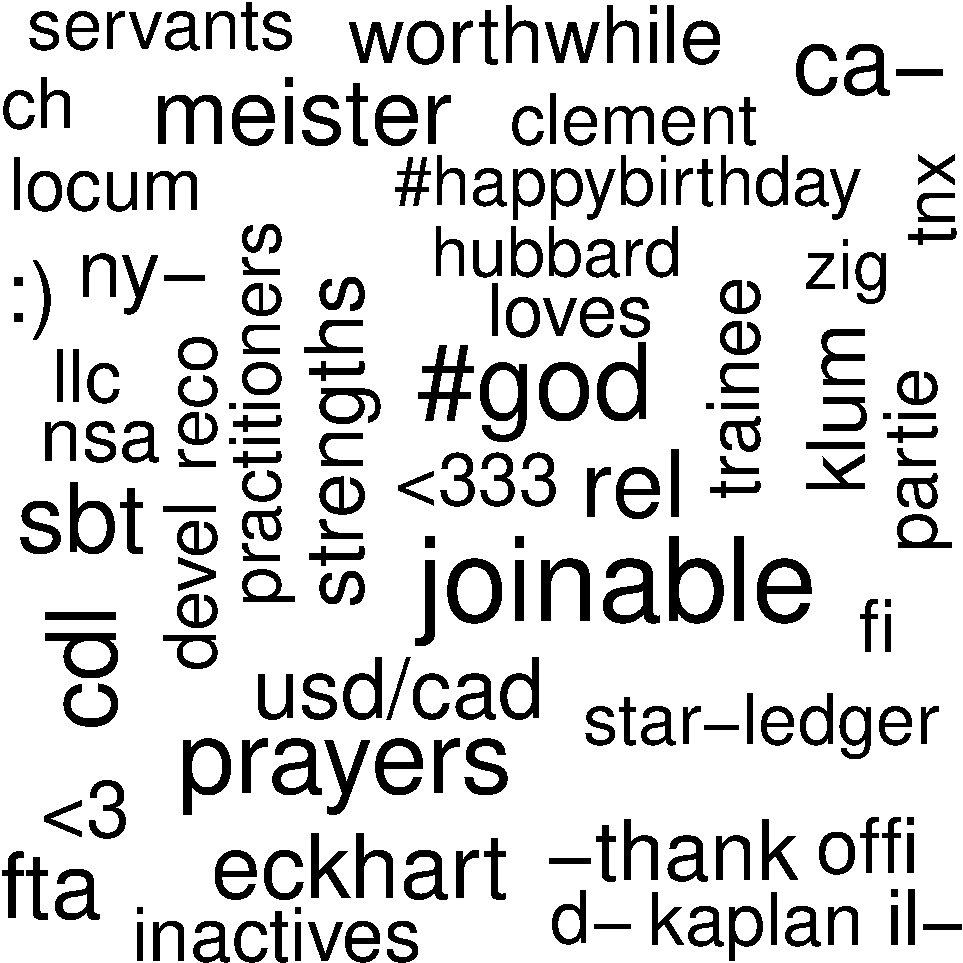
\includegraphics[scale=0.2]{pics/trust.pdf} \\
joy & sadness & surprise & trust\\
\end{tabular}}
\end{center}
\end{figure}

\end{scriptsize}
\end{frame}

\begin{frame}{Transfer Learning with Tweet Centroids}

\begin{figure}[htb]
	\centering
	 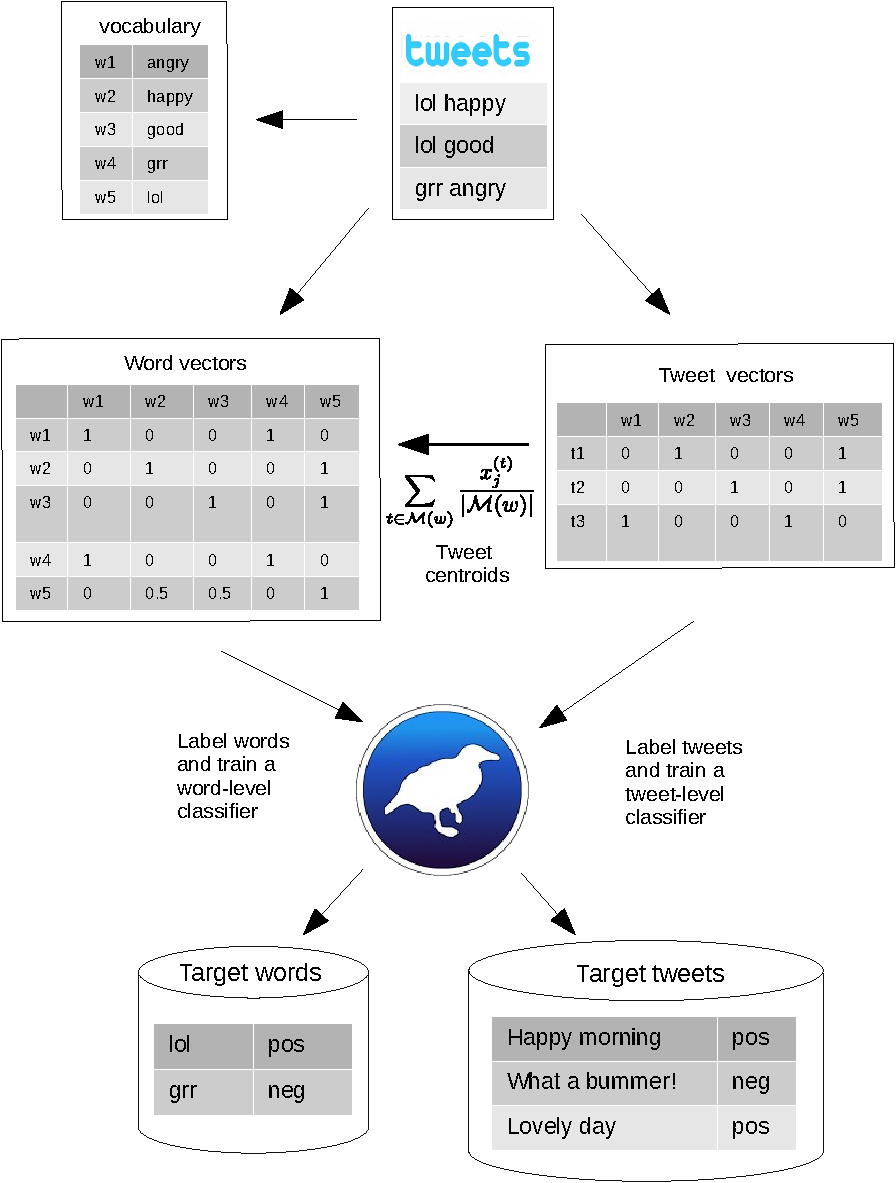
\includegraphics[scale=0.4]{pics/tweetsToWords.pdf}
\end{figure}



\end{frame}









\begin{frame}{Post PhD Projects}

\begin{enumerate}
 \item AffectiveTweets: and open source project for analyzing affect from social media posts (it has been used in around 30 publications and its website receives around 10 unique visits per day).
 \item Emotion Intensity Detection.
 \item Hate Speech Detection with deep neural networks.
 \item Time-evolving word vectors.
 \item Learning compatible representations between words and tweets.
 \item M\={a}ori loanwords on Twitter.
 \end{enumerate}

\end{frame}





\section{Academic Plan}


\begin{frame}{Goals at DCC}
\begin{scriptsize}
  \begin{enumerate}
\item Participate in the education of a new generation of Chilean computer scientists and artificial intelligence (ML and NLP) experts.
\item To teach existing courses, create new courses, and supervise undergraduate and postgraduate students' research projects. 
\item To position the department as a leading  center of NLP research in the region (actively publish in good NLP conferences and Journals\footnote{I am aware that ISI journals are very important in Chile.}, attract talented students to study with us as well as bringing collaborators to visit the department).
\item I believe that NLP and machine learning can be applied to various areas developed in the Department (e.g., Data Science, Algorithms, Software Engineering).
\item Help boosting the local industry and the public sector in AI, ML, and NLP.
\item Contribute to the internationalization of the department (teach courses in English?). 
  \end{enumerate} 
\end{scriptsize}

\end{frame}


\begin{frame}{Teaching Proposal}
\begin{scriptsize}
My main teaching goal is to create two regular courses to be taught to both undergraduate and postgraduate students
\begin{enumerate}
 \item A course on Natural Language Processing (NLP)
 \item A course  on Machine Learning (ML)
  \end{enumerate} 


\begin{itemize}
 \item I would also like to teach more advanced courses for postgraduate students about deep learning (neural networks that learn representations) and specific areas of NLP such as lexical semantics and sentiment analysis.
 \item Other topics I would be happy to teach: artificial intelligence, programming, programming methods, databases, algorithms and data structures, statistics, data mining, and information retrieval.  
\end{itemize}

\end{scriptsize}

\end{frame}


\begin{frame}{Research Proposal}
\begin{scriptsize}

\begin{itemize}
 \item Develop the intersection of stream machine learning and natural language processing. 
 \item Learn time-evolving representations for text using both distributional approaches and neural networks.
 \item Detect semantic change using change detectors (e.g., ADWIN).
 \item Learn universal representations for different types of objects (e.g., tweets, words, user) to transfer knowledge between domains.
 \item Create linguistic resources for low-resource indigenous languages (e.g., M\={a}ori, Mapudungun, Quechua)
 \item Apply for a FONDECYT initiation grant. 
\end{itemize}
\end{scriptsize}

\end{frame}





\begin{frame}
\frametitle{Questions?}
%\vspace{1.5cm}
\begin{center}\LARGE Thanks for your Attention!\\  \end{center}



\end{frame}




%%%%%%%%%%%%%%%%%%%%%%%%%%%

\end{document}
